\documentclass{article}

\usepackage{graphicx}
\usepackage{tikz}
\usepackage{tikzsymbols}
\usetikzlibrary{calc,patterns,shapes.geometric}
\pagestyle{empty}
\usepackage[margin=0pt]{geometry}
\geometry{papersize={14in,12in}}

\def\centerarc[#1](#2)(#3:#4:#5){\draw[#1] ($(#2)+({#5*cos(#3)},{#5*sin(#3)})$) arc (#3:#4:#5);}

\begin{document}
	\begin{figure}
		\centering
		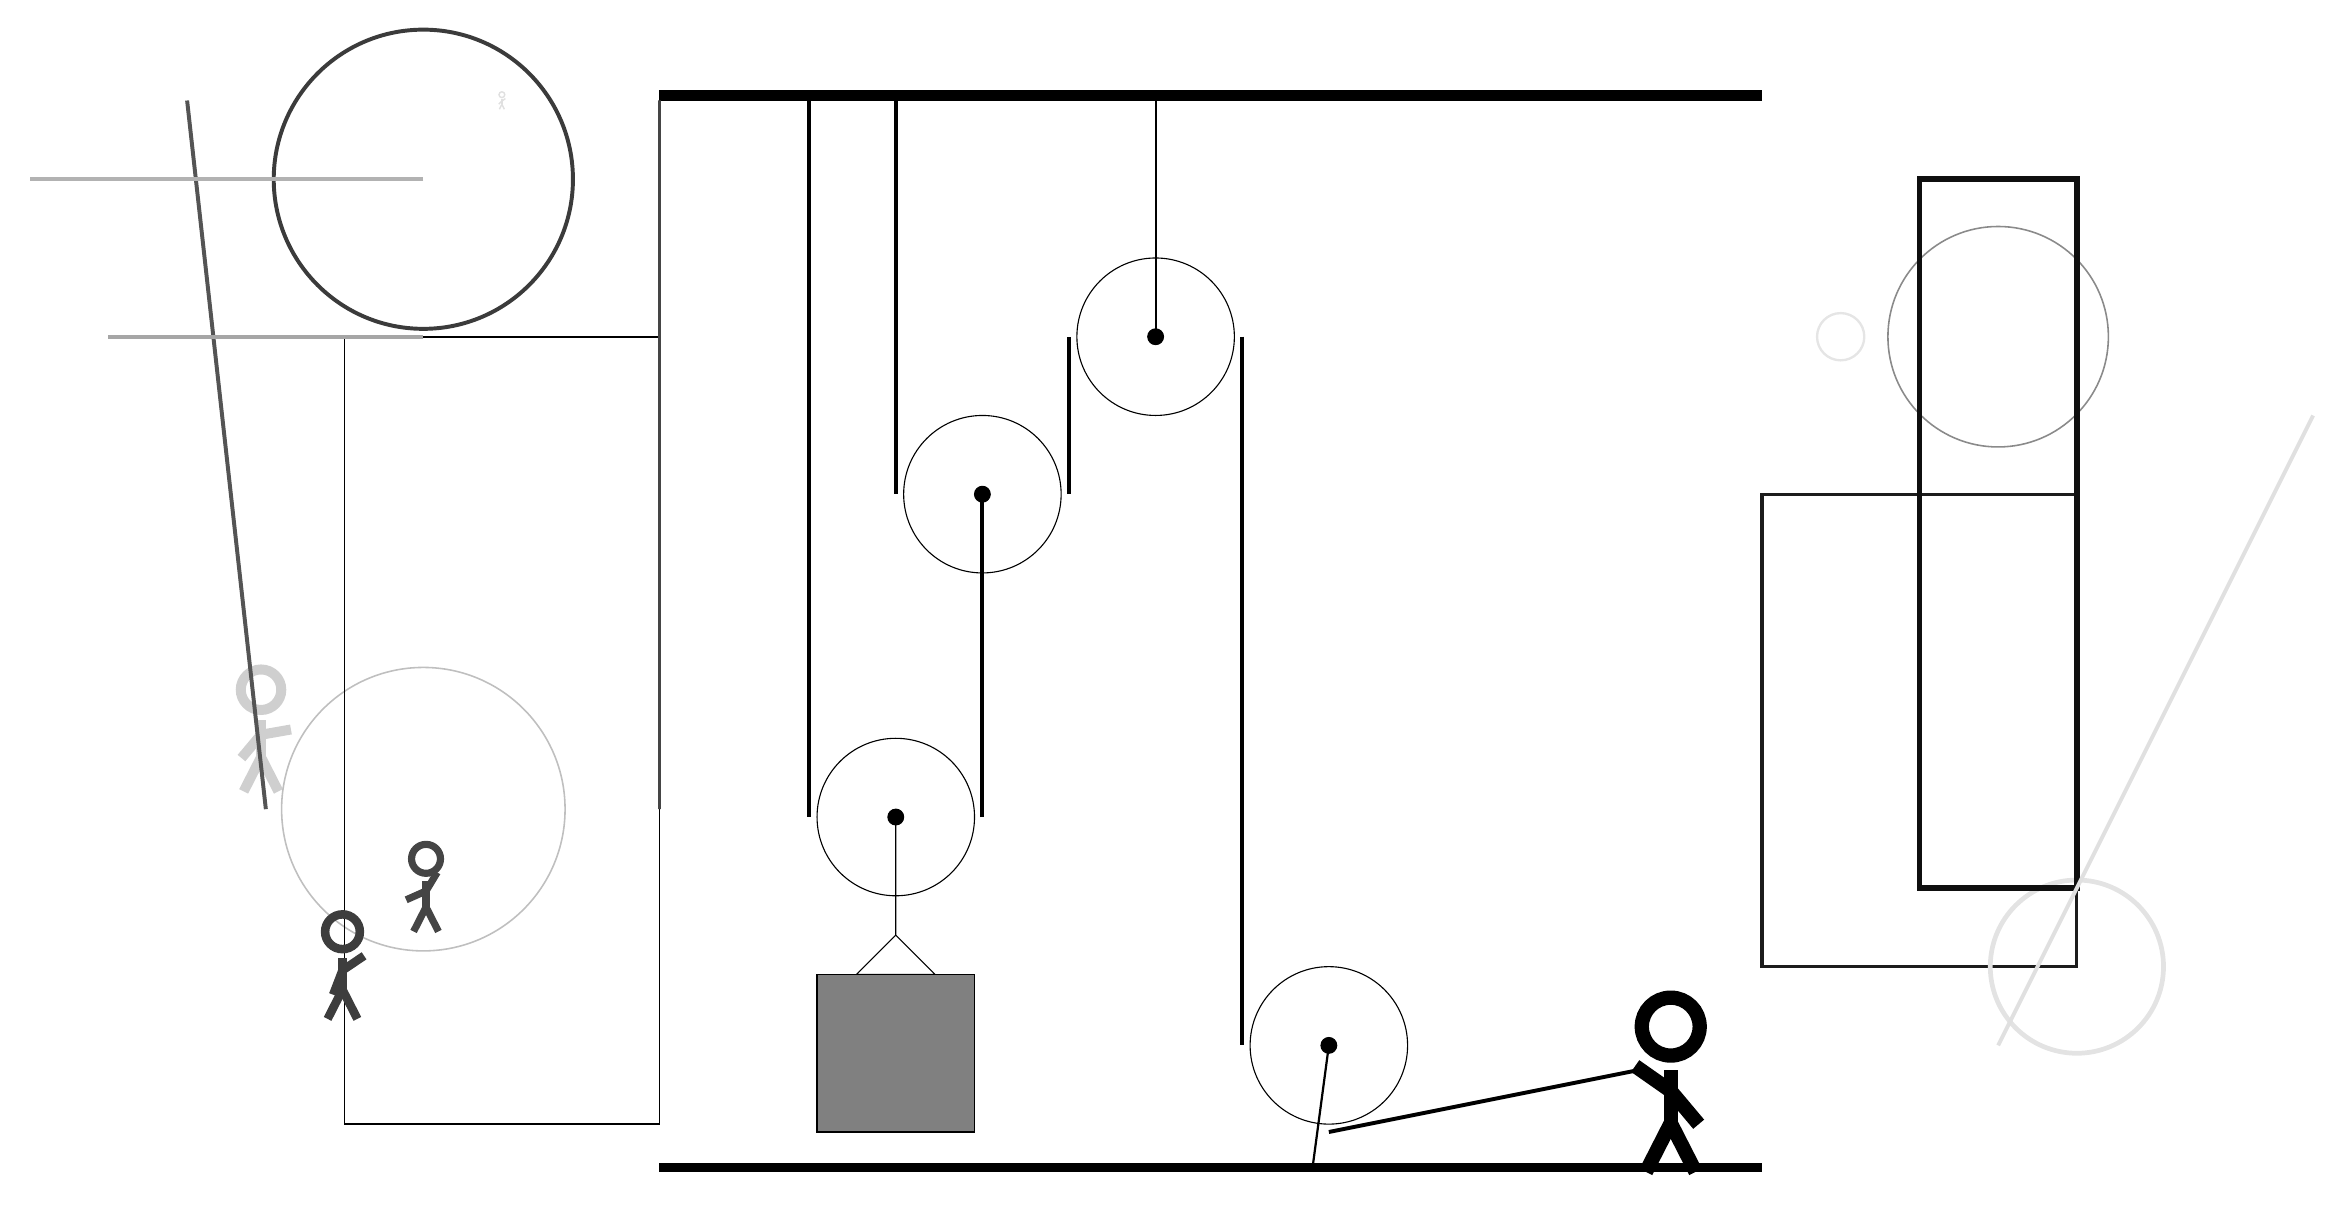
\begin{tikzpicture}
			%%%%% START %%%%%
			
			\draw[fill=black] (-2, 10) rectangle (12, 10.125);
			
			\draw (1, 0.9) circle (1);
			\draw[fill=black] (1, 0.9) circle (0.1);
			
			\draw (2.1, 5.0) circle (1);
			\draw[fill=black] (2.1, 5.0) circle (0.1);
			
			\draw (4.3, 7.0) circle (1);
			\draw[fill=black] (4.3, 7.0) circle (0.1);
			\draw[thick] (4.3, 7.0) -- (4.3, 10);
			
			\draw (6.5, -2) circle (1);
			\draw[fill=black] (6.5, -2) circle (0.1);
			\draw[thick] (6.5, -2) -- (6.3, -3.5);
			
			\draw (1, 0.9) -- (1, -0.6) -- (0.5, -1.1) -- (1.5, -1.1) -- (1, -0.6);
			\draw[fill=black!50] (0, -1.1) rectangle (2, -3.1);
			\draw[line width=0.5mm] (-0.1, 10) -- (-0.1, 0.9);
			\centerarc[line width=0.5mm](1, 0.9)(180:360:1.1);
			\draw[line width=0.5mm](2.1, 0.9) -- (2.1, 5.0);
			\draw[line width=0.5mm] (1.0, 10) -- (1.0, 5.0);
			\centerarc[line width=0.5mm](2.1, 5.0)(180:360:1.1);
			\draw[line width=0.5mm](3.2, 5.0) -- (3.2, 7.0);
			\centerarc[line width=0.5mm](4.3, 7.0)(0:180:1.1);
			\draw[line width=0.5mm] (5.4, 7.0) -- (5.4, -2);
			\centerarc[line width=0.5mm](6.5, -2)(0:90:-1.1);
			\draw[line width=0.5mm](6.5, -3.1) -- (10.5, -2.3);
			
			\node[line width=0.2mm, color=black!73] at (-5, 0) {\Strichmaxerl[5][24][59]};
			
			\draw [line width=0.5mm, color=black!77](-5, 9) circle (1.9);
			\node[line width=0.6mm, color=black!19] at (-7, 2) {\Strichmaxerl[7][50][10]};
			\draw [line width=0.2mm, color=black!25](-5, 1) circle (1.8);
			\draw[line width=0.2mm, color=black!100] (-2, 7) rectangle (-6, -3);
			\draw[line width=0.4mm, color=black!89] (12, -1) rectangle (16, 5);
			
			\draw[line width=0.5mm, color=black!67](-7, 1) -- (-8, 10);
			
			\draw [line width=0.3mm, color=black!10](13, 7) circle (0.3);
			\draw[line width=0.5mm, color=black!30](-5, 9) -- (-10, 9);
			
			\draw[line width=0.4mm, color=black!73] (-2, 10) rectangle (-2, 1);
			\draw [line width=0.2mm, color=black!46](15, 7) circle (1.4);
			\node[line width=0.5mm, color=black!12] at (-4, 10) {\Strichmaxerl[1][44][36]};
			\draw[line width=0.5mm, color=black!35](-5, 7) -- (-9, 7);
			
			\node[line width=0.7mm, color=black!76] at (-6, -1) {\Strichmaxerl[6][69][34]};
			\draw [line width=0.6mm, color=black!11](16, -1) circle (1.1);
			\draw[line width=0.7mm, color=black!94] (14, 9) rectangle (16, 0);
			
			\draw[line width=0.5mm, color=black!12](15, -2) -- (19, 6);
			
			\node at (10.8, -2.5) {\Strichmaxerl[10][-35][-50]};
			
			\draw[fill=black] (-2, -3.5) rectangle (12, -3.6);
			
			%%%%% END %%%%%
		\end{tikzpicture}
	\end{figure}	
\end{document}